In this section, we focus on Phase I of our framework and introduce our approach for feature augmentation. We propose a new perspective for transfer learning in HTL and analyze the reason why negative transfer could happen.

\subsection{Feature augmentation in HTL}
We define our transfer task in the following way: suppose we have $N$ visual categories. 
In our source task, $N$ source binary classifiers $f'_n(x)$ for $n=1,...,N$, are trained from a distribution $\mathcal{D}_s$ to distinguish whether an object belongs to each of the $N$ categories. In our target task, we have another small dataset $(x,y)$ drawn from another distribution $\mathcal{D}_t$ with the same $N$ categories as those in source task. We want to train $N$ target binary classifiers $f_n(x)$ for $n=1,...,N$ using this small target dataset so that they can perform well on future data of the target domain.

Vapnik et al. \cite{vapnik2015learning} proposed a diagram to transfer the \textit{privileged knowledge} from the teacher to the student. The privileged knowledge is used as the auxiliary feature for training the student model. Inspired by this idea, we propose our feature augmentation approach for HTL in domain adaptation. We treat the outputs of the source models as the auxiliary features and use them to train the target model. The difference between the auxiliary feature in our work and the privileged information is that we can use the auxiliary feature in both training and testing procedures while by assumption, privileged knowledge can only be used for training.

\begin{figure*}
	\centering
	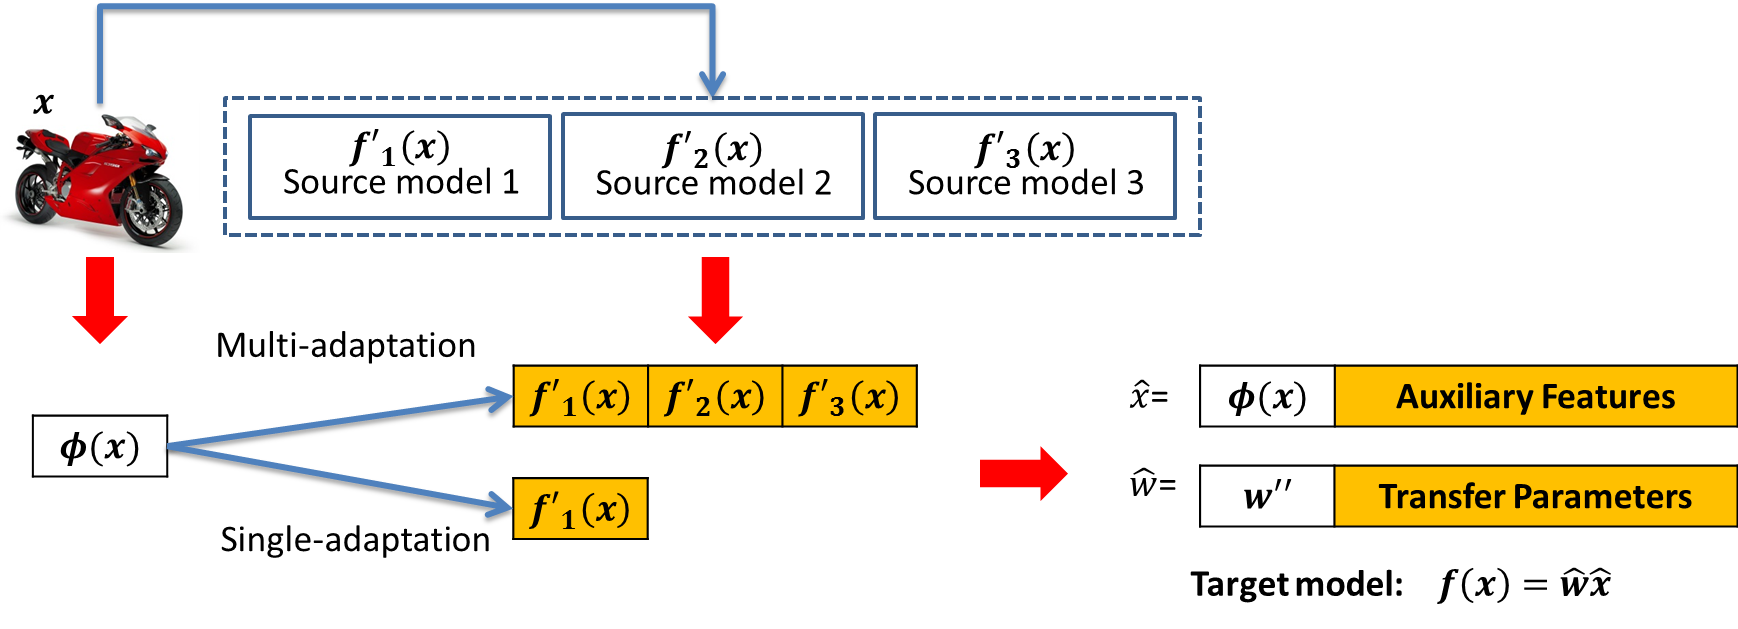
\includegraphics[scale=0.5]{fig/aug2.png}
	\caption{The transfer learning process can be considered as the augmentation of the target data where the decision scores of the source models are appended as the auxiliary features. The transfer parameters can be considered as a part of the corresponding hyperplane. We can consider 2 augmentation strategies: multi-adaptation and single-adaptation.}\label{fig:aug}
\end{figure*}

Inspired by \cite{vapnik2015learning}, when there are a group of $N$ source models $F'(x)=\{f'_i(x)|i=1,...,n\}$, we can augment the target feature space as  $\hat{x}=[\phi(x),f'_1(x),...,f'_N(x)]$ when we want to leverage the knowledge from multiple source models (Multi-adaptation) or $\hat{x}=[\phi(x),f'_r(x)], r\in 1,...,N$ (Single-adaptation). Here $\phi(x)$ can be any feature mapping that maps the example into another space. Thus the target binary model for category $n$ can be represented as $f_n=\hat{w}_n\hat{x}$, where $\hat{w}_n=[w_{n}'',\beta_1,...,\beta_N]$ (Multi-adaptation) or $[w_{n}'',\beta_r]$ (Single-adaptation). Here, we call $\beta$ the \textit{Transfer Parameter}.

\begin{equation}\label{eq:aug_pre}
\begin{aligned}
f_n(x)&=w_{n}''\phi(x)+\sum\limits_k^N{\beta _kw'_k\phi(x)}
\end{aligned}
\end{equation}
An intuitive interpretation of Eq. \eqref{eq:aug_pre} is that, when the target model decides whether an object belongs to a certain category, it also considers the decisions of the source models as a reference (the second part of the right hand side in Eq. \eqref{eq:aug_pre}). The transfer parameter $\beta$ here is to control the weight of the decision from the source model, i.e. the amount of the knowledge transferred from the source domain.

The best $f_n$ can be found by solving the following optimization problem:
\begin{equation}\label{eq:svm_obj}
\begin{aligned}
\textbf{min} && \Omega({w}_n) + \frac{C}{2}\sum\limits_i^l {\mathcal{L}(f_n(x_i),Y_{in})} \\
\end{aligned}
\end{equation}
Here $\Omega({w})$ is the regularization term to encourage good generalization performance and avoid overfitting. $Y_{in}$ is the encoded label for binary classifier following $Y_{in}=1$ if $y_i=n$ and $-1$ otherwise. $\mathcal{L}(\cdot)$ is the loss function. When we consider to use Least Square SVM as the classifier, we have $\mathcal{L}(f,y) = (f-y)^2$ and $\Omega({w}) = \frac{1}{2}||w||^2$. 

Apparently, $\hat{w}$ can be solved directly by minimizing the optimization problem \eqref{eq:svm_obj}. However, if we are not able to regularize $\hat{w}$ properly, the target model could easily suffer from negative transfer when the source and target are weakly related (see the experiment result for the method Feature+ in Section \ref{sec:exp}).  

Compared to the previous methods in HTL \cite{tommasi2014learning} \cite{aytar2011tabula}, we have the following advantages:
\begin{itemize}
	\item Wider range selection of the source model. Most of the previous works in HTL only support the linear source model \cite{tommasi2014learning} \cite{aytar2011tabula}. With the idea of feature augmentation, we only require the source model to be a function that can output the decision score of an example. Therefore, we can exploit the knowledge of the different types, such as Neural Networks and inference models \footnote{Previous works, such as \cite{tommasi2014learning} \cite{aytar2011tabula}, can be considered as the special case of our problem where the linear model is used as the source. We can obtain similar objective function when we consider the transfer parameter as the hyper-parameter that can be defined according to the background knowledge.}.
	\item Insight into the performance of the target model. By feature augmentation, we turn the HTL domain adaptation problem into a classical learning problem and we can better analyze some important issues existed in transfer learning such as negative transfer. In the next subsection, we show the statistical analysis of how to improve the performance of the target model in our framework. 
\end{itemize}

\subsection{Statistical analysis of the feature augmentation}
From the perspective of the feature augmentation, we can turn the problem of domain adaptation with HTL into a traditional learning problem, i.e. to find the optimal values for the elements of the hyperplane hyperplane $\hat{w}=[w_{n}'',\beta_1,...,\beta_N]$ \footnote{We take Mult-adaptation for instance. The conclusion can be applied to Single-adaptation without any modification.}. According to the principle of Structural Risk Minimization (SRM) \cite{vapnik1999overview}, the risk of a linear classifier $f(x)=wx$ on the unseen test data $R(f)$ (generalization risk) is bounded by:
\begin{equation}\label{eq:srm}
R(f) \le {R_{emp}}(f) + \mathcal{O}\left(\sqrt{\frac{h}{l}}\right)%\sqrt {\frac{{h(\ln (2l/h) + 1) + \ln (\delta /4)}}{l}} 
\end{equation}
Here the first part on the right-hand side of the inequation ${R_{emp}}(f)$ is the empirical risk (training error) of the classifier and the second part is the confidence interval. $h$ and $l$ denote the VC dimension and number of training data of the classifier, respectively. According to \cite{suykens1999least}, the VC dimension $h$ is bounded by $h \le \min([||w||^2R^2],m)+1$ where $R$ and $m$ is the radius of the smallest ball containing data $x$ and the dimension of $x$. $||w||$ is the \textit{2-norm} of the hyperplane.

As we discussed above, we use the outputs of the source models as the auxiliary features to augment the target data. Let $R$ and $\hat{R}$ denote the radius of the data before and after augmentation. We should have $R^2 \le \hat{R}^2$. When the auxiliary features can't provide any useful information to reduce the empirical risk $R_{emp}(f)$, i.e. the source model is unrelated if we failed to limit $||\hat{w}||^2$, the VC dimension $h$ will increase. Thus, the generalization risk $R(f)$ would increase and the target model suffers from negative transfer. For example, when the source models are unrelated, the optimal solution is to set the transfer parameters to 0s which is equivalent to the method without transferring any source knowledge (no transfer model). In contrast, if we can significantly decrease the empirical risk $R_{emp}(f)$ of the target model trained on the augmented data (augmented model), even though its VC dimension $h$ increases, its generalization risk still decreases and the augmented model can get improved performance, i.e. positive transfer.

From the analysis above, we can see that in order to get improved performance and alleviate negative transfer, we should evaluate the source models and carefully set the values of the transfer parameters to control the amount of knowledge from the source models. The optimal values of the transfer parameters should be able to control the VC dimension $h$ and reduce the empirical risk $R_{emp}(f)$ simultaneously.
In next section, we introduce our method SMTLe to estimate the transfer parameters that can improve the performance of the target model and alleviate negative transfer .

